\documentclass[14pt,a4paper]{extarticle}

\usepackage{fontspec}
\setmainfont{Times New Roman}[Ligatures=TeX]
\setmonofont{Courier New}
\newfontfamily\cyrillicfonttt{Courier New}

\usepackage{polyglossia}
\setmainlanguage{russian}
\setotherlanguage{english}

\usepackage{geometry}
\geometry{left=30mm,right=15mm,top=20mm,bottom=20mm,headheight=0pt,headsep=0pt}

\usepackage{setspace}
\onehalfspacing
\usepackage{indentfirst}
\setlength{\parindent}{1.25cm}

\usepackage{titlesec}
\titleformat{\section}{\normalsize\bfseries\centering}{\thesection.}{0.5em}{}
\titleformat{\subsection}{\normalsize\bfseries}{\thesubsection.}{0.5em}{}
\titlespacing*{\section}{0pt}{1.25em}{0.8em}
\titlespacing*{\subsection}{0pt}{1.05em}{0.55em}

\usepackage{graphicx}
\graphicspath{{figures/}}
\usepackage{caption}
\captionsetup{font=small,skip=8pt,justification=centering}
\usepackage{enumitem}
\setlist[itemize]{leftmargin=1.25cm,itemsep=0.2em,topsep=0.35em,parsep=0pt}
\setlist[enumerate]{leftmargin=1.25cm,itemsep=0.2em,topsep=0.35em,parsep=0pt}

\usepackage{pdfpages}
\usepackage{hyperref}
\hypersetup{hidelinks,unicode,pdftitle={Обзор системы валидации юридического лица для получения кредита}}

\setlength{\parskip}{0pt}
\clubpenalty=10000
\widowpenalty=10000
\emergencystretch=3em

\begin{document}

\IfFileExists{first_page.pdf}{%
\includepdf[pages=1,pagecommand={\thispagestyle{empty}}]{first_page.pdf}%
}{%
\begin{titlepage}
\thispagestyle{empty}
\begin{center}
МИНИСТЕРСТВО НАУКИ И ВЫСШЕГО ОБРАЗОВАНИЯ\\
РОССИЙСКОЙ ФЕДЕРАЦИИ

\vspace{0.8em}
ФЕДЕРАЛЬНОЕ ГОСУДАРСТВЕННОЕ АВТОНОМНОЕ\\
ОБРАЗОВАТЕЛЬНОЕ УЧРЕЖДЕНИЕ ВЫСШЕГО ОБРАЗОВАНИЯ

\vspace{0.7em}
{\bfseries НАЦИОНАЛЬНЫЙ ИССЛЕДОВАТЕЛЬСКИЙ\\ ЯДЕРНЫЙ УНИВЕРСИТЕТ «МИФИ»}

\vspace{1.6em}
Институт интеллектуальных кибернетических систем\\
Кафедра кибернетики (№~22)

\vspace{0.8em}
Направление подготовки 09.04.04\\ Программная инженерия

\vspace{1.6em}
Курсовая работа\\
по моделированию предметных сред\\
и проектированию баз данных

\vspace{1.4em}
{\bfseries «Проектирование информационной системы\\ валидации юридического лица\\ для получения кредита»}

\vspace{0.6em}
Раздел 1. Обзор системы
\end{center}

\vspace{1.6em}
\hfill
\begin{minipage}{0.62\textwidth}
Выполнил студент группы М26-514\\
Гришанов~Н.\,В.\\[0.9em]
Преподаватель\\
Тихомирова~Д.\,В.
\end{minipage}

\vfill
\begin{center}
Москва 2026
\end{center}
\end{titlepage}
}

\renewcommand{\contentsname}{Содержание}
\tableofcontents
\newpage

\section{Обзор системы}

\subsection{Формулировка задания}

Необходимо спроектировать информационную систему валидации юридического лица для получения кредита. Система проверяет организацию по законодательству Российской Федерации и по кредитным условиям банка и завершает работу заключением. Заключение передаётся контуру выдачи. Договор, график платежей и зачисление остаются за границей системы. Период охлаждения потребительского кредита к проверке юридического лица не относится.

Организация подаёт заявку с суммой, сроком, валютой и целью. Вместе с заявкой учитываются люди, которые в ней участвуют, цепочка владения между юридическими лицами, обязательные проверки и показатели, сопоставленные с условиями продукта. Вывод по показателю~--- усиливает, ослабляет или блокирует~--- хранится в связи <<Учтено>> вместе с применённым весом и порогом. Обязательная проверка фиксирует соответствие норме. Срок хранения зависит от категории сведений: клиент, показатель, пакет заявки и кредитные условия живут отдельно.

\subsection{Назначение и цели создания системы}

Назначение~--- проверять юридическое лицо для получения кредита по одним правилам в офисе и в дистанционном канале. Карточка организации, согласия, проверки, показатели и условия общие для менеджера и автоматической проверки.

Цели:

\begin{enumerate}
\item учёт организации, участия людей и владения между организациями;
\item фиксация согласия лица и организации на обработку сведений и на запрос кредитной истории;
\item обязательные проверки по норме с источником и датой;
\item учёт показателей в заявке: вес, порог и вывод по условиям этой заявки;
\item заявка на одних кредитных условиях, с корпоративным одобрением и обеспечением, когда сделка этого требует;
\item заключение с результатом, уровнем риска, сроком действия и причиной отказа;
\item четыре категории хранения: клиент, показатель, пакет и условия.
\end{enumerate}

\subsection{Основные функциональные возможности системы}

Учёт юридического лица. Наименование и организационно-правовая форма, ИНН, ОГРН и ОКВЭД, статус, адрес, лицензия. Статус и лицензируемый вид деятельности читаются из карточки организации.

Учёт физического лица и участия. ФИО, паспорт и дата рождения, гражданство и адрес. Участие хранит долю, вид связи и основание. Виды связи: учредитель, руководитель, бенефициар, представитель. Бенефициарный владелец~--- физическое лицо с долей более двадцати пяти процентов либо с возможностью контролировать организацию. Если такое лицо не установлено, для идентификации берётся единоличный исполнительный орган.

Владение. Связь двух юридических лиц: доля и основание. Одна сторона~--- владелец, другая~--- объект владения. Косвенная доля считается произведением долей по цепочке. Человек владеет шестьюдесятью процентами организации, а та~--- сорока процентами другой: косвенная доля во второй организации составляет двадцать четыре процента. Порог бенефициарного владения~--- более двадцати пяти процентов либо контроль, и во второй организации он не пройден. В первой организации этот человек~--- бенефициарный владелец. Промежуточная организация остаётся стороной владения.

Согласие. Цель обработки, основание и срок действия. Согласие даёт физическое лицо или юридическое лицо. Проверка ссылается на согласие, когда использует персональные данные или кредитную историю. Срок действия согласия хранится в самом согласии и срок хранения записи не заменяет.

Обязательная проверка. Вид и норма, результат, источник и дата. Проверка принадлежит заявке. Связь <<по лицу>> необязательна и нужна для полномочий, бенефициара и публичного должностного лица. Результат~--- пройдена или не пройдена. Непройденная проверка закрывает путь к положительному заключению. Вес у правовой проверки отсутствует: норма либо соблюдена, либо нет.

Финансовая отчётность и показатель. Организация ведёт отчёты: форма, период, валюта, дата составления. Отчёт содержит показатели. Показатель хранит вид и период, значение, источник и дату и может быть записан без отчёта, если источник~--- суд, налог или бюро. В заявку показатель попадает через связь <<Учтено>>: вес, порог и вывод. Вывод относится к этой заявке и этим условиям. Новая редакция условий оставляет уже записанный вес прежним.

Заявка и кредитные условия. Номер, дата и канал, сумма, срок и валюта, статус и цель проверки. Каналы: интернет-банк, офис, менеджер. Цели: первичное рассмотрение, увеличение лимита, пролонгация, замена обеспечения. Заявка ссылается ровно на одни кредитные условия: продукт и валюта, лимиты и срок, требование обеспечения. Новая редакция лимитов~--- новая запись условий. Повторная проверка~--- новая заявка.

Корпоративное одобрение. Орган и дата решения, вид сделки, одобренная сумма. Вид сделки~--- крупная сделка или сделка с заинтересованностью. Одобрение есть не у каждой заявки.

Обеспечение. Вид и предмет залога, оценка стоимости, действующее обременение. Заявка предлагает ноль или несколько обеспечений, когда условия продукта этого требуют.

Заключение. Результат проверки, уровень риска, срок действия, причина отказа. У заявки ноль или более заключений. Результат: положительный, положительный с ограничениями, отказ. Риск: низкий, средний, высокий, критический. Пересмотр добавляет новое заключение и сохраняет предыдущее. Связь заключения с показателем проходит через заявку и через <<Учтено>>.

Правило хранения. Категория сведений, основание и срок, событие начала отсчёта. Категория <<клиент>> покрывает физическое и юридическое лицо; участие и владение хранятся вместе с ними. Категория <<показатель>> покрывает показатель и финансовую отчётность. Категория <<пакет>> покрывает заявку, проверку, связь <<учтено>>, корпоративное одобрение, обеспечение и заключение. Категория <<условия>> покрывает редакции кредитных условий.

\subsection{Конкретизация предметной области}

Предметная область~--- проверка организации до заключения по заявке на заданных условиях. Модель приведена на рисунке~\ref{fig:kmpo}. Синий блок~--- данные предметной области, красный~--- контроль обработки и хранения, ромб~--- связь с собственными атрибутами. Знак у сущности задаёт её кратность: черта~--- ровно один, круг~--- ноль или один, круг и лапка~--- ноль или много, черта и лапка~--- один или много. Связи правила хранения на рисунке не проведены: четыре категории и их состав записаны в легенде.

\begin{figure}[p]
\centering
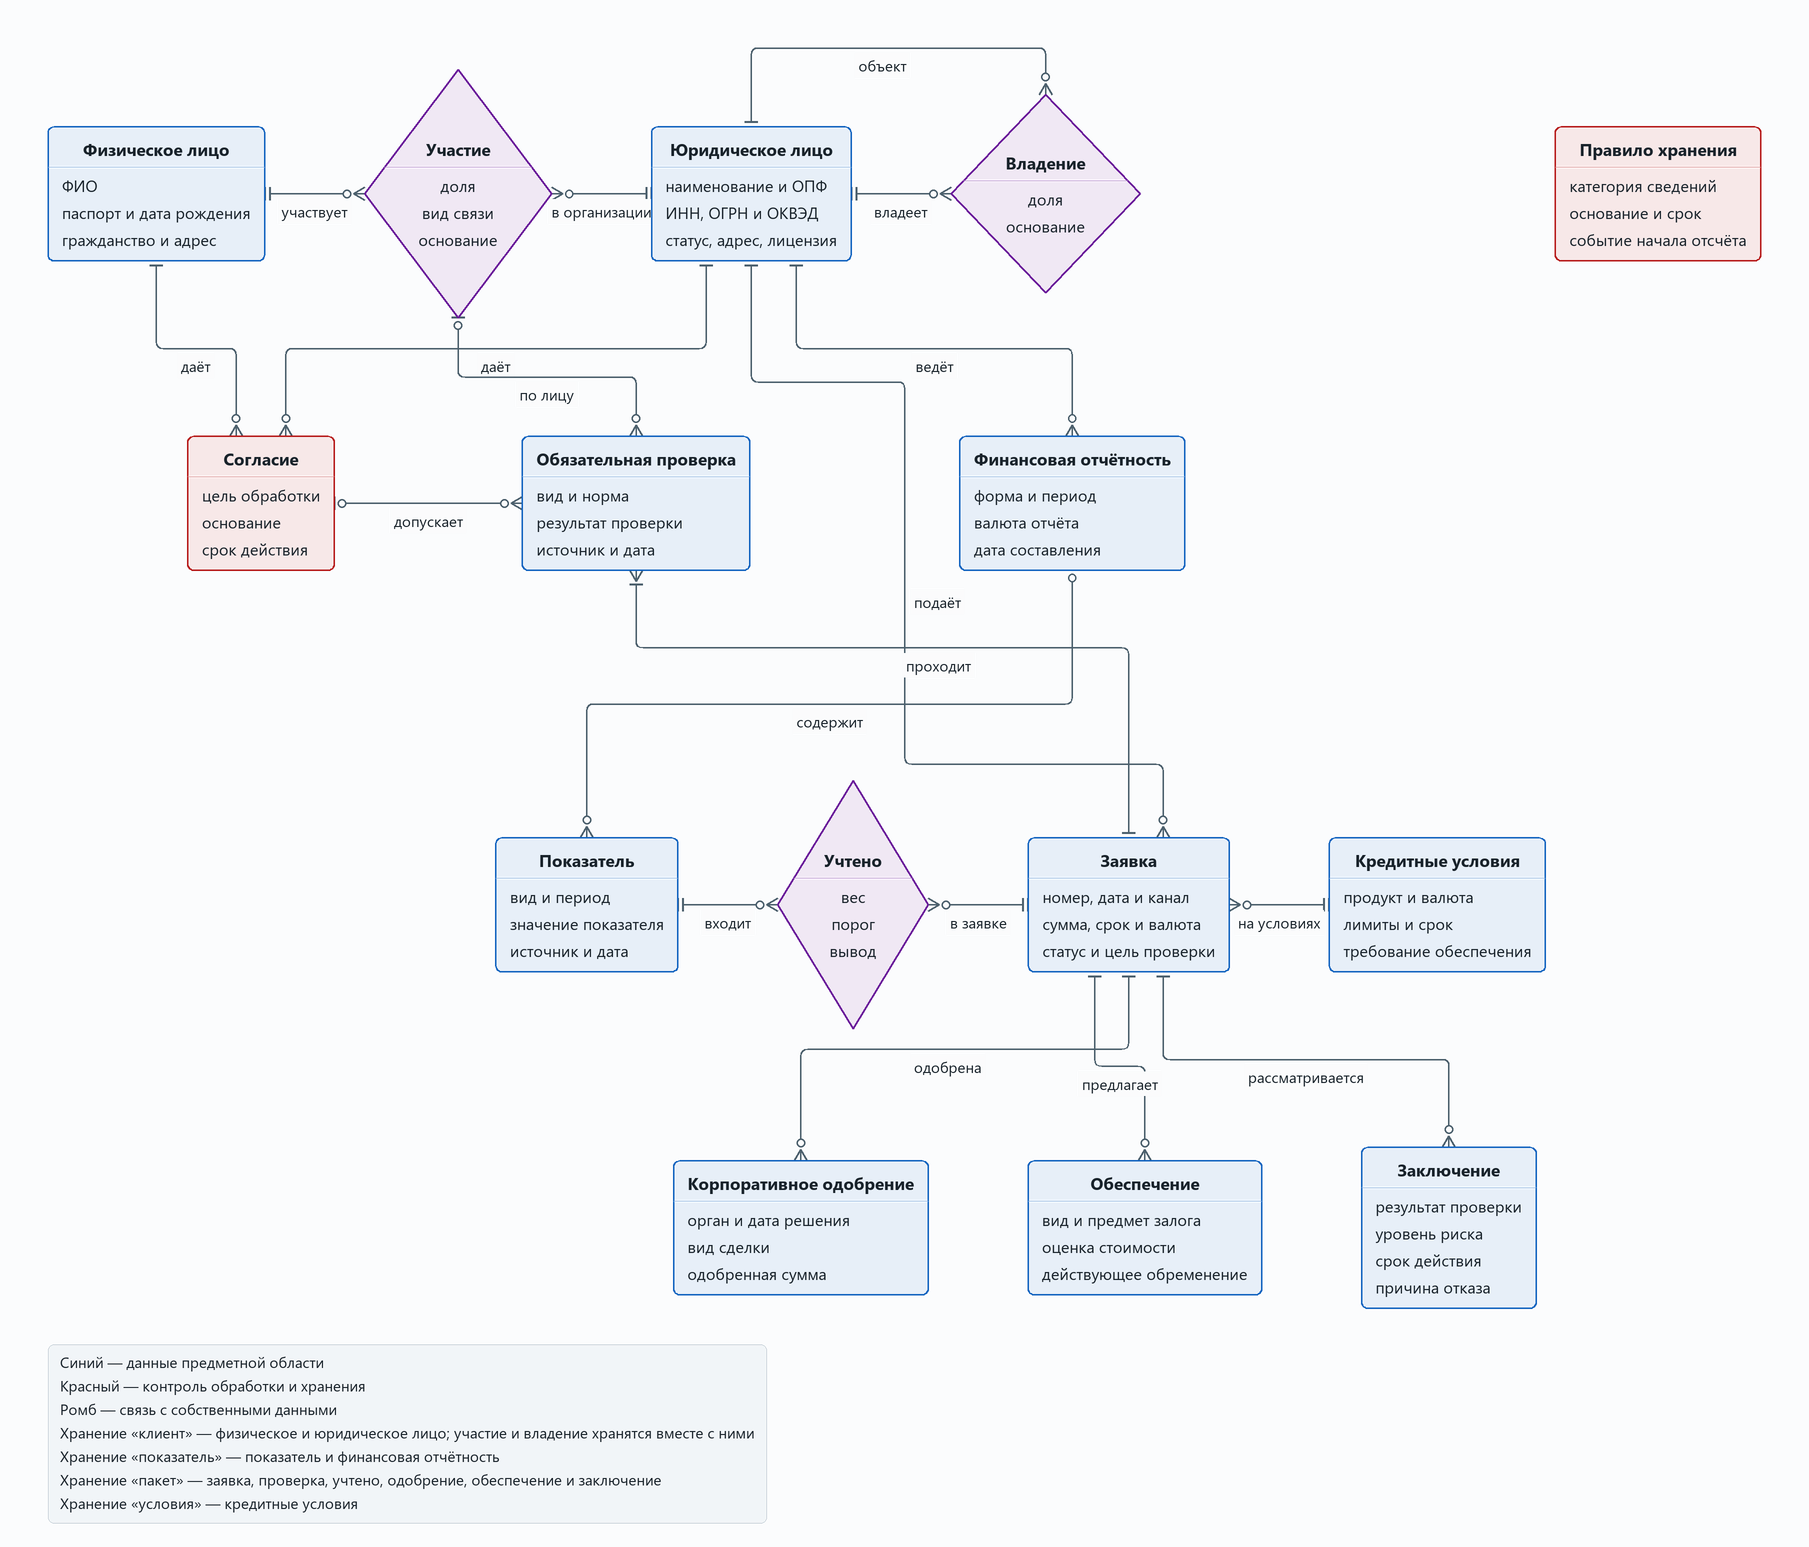
\includegraphics[width=\textwidth]{kmpo_validaciya.png}
\caption{Концептуальная модель предметной области валидации юридического лица для получения кредита}
\label{fig:kmpo}
\end{figure}

Физическое лицо. ФИО, паспорт и дата рождения, гражданство и адрес. Связь <<участвует>>: у участия ровно одно лицо, у лица~--- ноль или много участий.

Участие. Доля, вид связи, основание. Связь <<в организации>>: участие принадлежит ровно одной организации, у организации~--- ноль или много участий. Участие без организации не создаётся.

Юридическое лицо. Наименование и организационно-правовая форма, ИНН, ОГРН и ОКВЭД, статус, адрес, лицензия. Подаёт нуль или более заявок; у заявки организация ровно одна.

Владение. Доля и основание. Связь <<владеет>> указывает организацию-владельца: у записи владения владелец ровно один. Связь <<объект>> указывает организацию, которой владеют: объект тоже ровно один. Одна организация выступает владельцем и объектом в разных записях, и из таких записей собирается цепочка.

Согласие. Красная контрольная сущность: цель обработки, основание, срок действия. Его даёт физическое лицо либо юридическое лицо. По связи <<даёт>> у согласия ровно один давший, у лица и у организации~--- ноль или много согласий.

Обязательная проверка. Вид и норма, результат проверки, источник и дата. Связь <<проходит>>: проверка принадлежит ровно одной заявке, у заявки одна или несколько проверок. Связь <<допускает>>: у проверки не более одного согласия. Связь <<по лицу>>: у проверки не более одного участия.

Финансовая отчётность. Форма и период, валюта отчёта, дата составления. Связь <<ведёт>>: отчёт принадлежит ровно одной организации. Связь <<содержит>>: у показателя не более одного отчёта, у отчёта~--- ноль или много показателей.

Показатель. Вид и период, значение показателя, источник и дата. Связь <<входит>>: у записи <<Учтено>> ровно один показатель. Связь <<в заявке>>: у этой записи ровно одна заявка, у заявки~--- ноль или много учтённых показателей. Вес, порог и вывод стоят на ромбе <<Учтено>>.

Заявка. Номер, дата и канал, сумма, срок и валюта, статус и цель проверки. Связь <<на условиях>>: у заявки ровно одни кредитные условия, у условий~--- ноль или много заявок.

Кредитные условия. Продукт и валюта, лимиты и срок, требование обеспечения. Общая рамка для заявок разных организаций. Срок жизни редакции задаёт категория хранения <<условия>>.

Корпоративное одобрение. Орган и дата решения, вид сделки, одобренная сумма. Связь <<одобрена>>: у одобрения ровно одна заявка, у заявки~--- ноль или много одобрений.

Обеспечение. Вид и предмет залога, оценка стоимости, действующее обременение. Связь <<предлагает>>: у обеспечения ровно одна заявка, у заявки~--- ноль или много предметов.

Заключение. Результат проверки, уровень риска, срок действия, причина отказа. Связь <<рассматривается>>: у заключения ровно одна заявка, у заявки~--- ноль или много заключений. Заключение существует только вместе с заявкой и действует до указанной даты.

Правило хранения. Красная контрольная сущность: категория сведений, основание и срок, событие начала отсчёта. На рисунке оно стоит отдельно. Легенда относит к категории <<клиент>> лицо, организацию, участие и владение; к категории <<показатель>>~--- показатель и отчётность; к категории <<пакет>>~--- заявку, проверку, <<учтено>>, одобрение, обеспечение и заключение; к категории <<условия>>~--- кредитные условия.

Первичная проверка собирает организацию, участие, при длинной цепочке~--- владение, нужные согласия, отчётность и показатели, заявку на одних условиях, обязательные проверки и записи <<Учтено>>, при необходимости одобрение и обеспечение, затем заключение. Повторная проверка добавляет новую заявку и новое заключение. Состав сущностей тот же.

\subsection{Пользователи системы}

Представитель юридического лица создаёт обращение, передаёт сведения об организации, лицах и долях и видит результат, срок и причину отказа по своей заявке.

Клиентский менеджер ведёт заявку, выбирает кредитные условия и отправляет заявку на проверку.

Кредитный аналитик вносит финансовую отчётность и показатели и записывает в связи <<Учтено>> вес, порог и вывод.

Андеррайтер выносит заключение по проверкам, учтённым показателям, условиям, одобрению и обеспечению.

Специалист финансового мониторинга ведёт участие и владение: долю, основание, руководителя, бенефициара и цепочку организаций.

Администратор правил хранения задаёт категорию, основание, срок и событие начала отсчёта.

Руководитель читает отчёты по заявкам, отказам и уровню риска.

Администратор системы заводит сотрудников и назначает роли.

\subsection{Сроки хранения информации}

Срок задаёт правило хранения: категория, основание, длительность и событие начала отсчёта. Ниже~--- проектные значения. Срок действия согласия является атрибутом согласия и эти сроки не подменяет. Запись о согласии хранится вместе с клиентом, который его дал.

Категория <<клиент>>. Физическое лицо, юридическое лицо, участие и владение~--- пять лет после прекращения отношений с клиентом. Основание~--- законодательство о противодействии отмыванию доходов.

Категория <<показатель>>. Показатель и финансовая отчётность~--- пять лет с даты показателя или с даты составления отчёта. Срок не равен сроку черновика заявки, в которой показатель впервые учли.

Категория <<пакет>>. Заявка, обязательные проверки, связь <<Учтено>>, корпоративное одобрение, обеспечение и заключения~--- пять лет с окончания срока заключения, с даты отказа или с даты, когда заявка истекла.

Категория <<условия>>. Редакция кредитных условий и сама запись правила~--- пять лет после того, как их перестали назначать новым заявкам. Уже созданные заявки сохраняют прежнюю ссылку.

Неотправленный черновик~--- один год с даты создания. Журнал действий сотрудников~--- пять лет.

\subsection{События, изменяющие состояние системы}

\begin{enumerate}
\item регистрация или обновление юридического лица: статус, адрес, ОКВЭД, лицензия;
\item идентификация физического лица и изменение участия;
\item появление или изменение записи владения между организациями;
\item выдача, отзыв или истечение согласия;
\item поступление финансовой отчётности и показателя;
\item результат обязательной проверки;
\item создание заявки, выбор условий и учёт показателя с весом, порогом и выводом;
\item корпоративное одобрение и предложение обеспечения;
\item заключение, его пересмотр, истечение срока, отказ или отмена заявки;
\item новая редакция условий или правила хранения;
\item создание, блокировка пользователя или смена роли.
\end{enumerate}

Первичная проверка проходит организацию, участие и при необходимости владение, согласия, показатели, заявку на условиях продукта, обязательные проверки, записи <<Учтено>> и заключение. Непройденная проверка или вывод <<блокирует>> дают отказ. Истечение срока делает заключение недействующим и сохраняет показатели, проверки и прежние заключения.

\subsection{Модель жизненного цикла системы}

Принята V-образная модель: требования и правила валидации, проектирование предметной области, базы и компонентов, затем модульные, интеграционные, системные и приёмочные испытания.

Правила проверяемы до кода. Положительный результат недоступен при непройденной обязательной проверке и при выводе <<блокирует>>. Заключение без срока действия не принимается. Заявка на проверке без обязательной проверки~--- дефект. Вес записывается в <<Учтено>> этой заявки и при новой редакции условий остаётся прежним. Косвенная доля равна произведению долей по цепочке владения, а бенефициарный владелец~--- физическое лицо. Одинаковые организация, показатели и условия дают один уровень риска в офисе и в интернет-банке.

Концептуальная модель этого раздела относится к системному проектированию. Следующие этапы сверяются с теми же кратностями и с теми же четырьмя категориями хранения.

\subsection{Выбор инструментальных средств проектирования}

Модели системы строятся в UML Studio. Это собственная система, написанная на Python. Текст диаграммы разбирается во внутреннюю модель и раскладывается послойным алгоритмом Сугиямы: снимаются циклы, узлам назначаются уровни, порядок в ряду подбирается так, чтобы сократить пересечения, связи проводятся ортогонально. Изображение собирает библиотека Pillow.

Сам UML используется через эту систему. В ней задаются концептуальная модель предметной области, диаграммы вариантов использования и состояний заявки и заключения, а также логическая и физическая модели: сущности, связи и кратности.

\end{document}
